\documentclass[twocolumn]{article}
\usepackage{amsmath}
\usepackage{graphicx}
\usepackage{subcaption}
\usepackage{fancyvrb}

\columnsep=2em

\title{Modularizing Street Map Generation \\
    \vspace{8pt} \large An Adventure in Tensors}
\author{William Clarkson \and Marcella Hastings \and Nathaniel Tenczar}
\date{\today}

\newcommand{\sqmat}[4]{\ensuremath{
    \left(\begin{array}{cc}
        #1 & #2 \\
        #3 & #4
    \end{array}\right)}}
\newcommand{\mkvec}[2]{\ensuremath{
    \left(\begin{array}{c}
        #1 \\
        #2 \\
    \end{array}\right)}}
\newcommand{\pt}{\textbf{p}}
\newcommand{\todo}[1]{\begin{center}\fbox{\parbox{150pt}{#1}}\end{center}}
\def \cpp {C\nolinebreak[4]\hspace{-.05em}\raisebox{.4ex}{\tiny\bf ++}~}

\begin{document}
\maketitle

\begin{abstract}
This paper addresses the issue of creating modular, extensible code to
implement a pipeline for procedurally modeling large street networks. We
describe a functional implementation of a framework that allows users to create
a realistic street network over an empty domain, based on the techniques
described in \textit{Interactive Procedural Street Modelling} by Chen et al.
\cite{chen}. In particular, we were able to express the underlying mathematics
more intuitively and clearly than is possible in an imperative language, and
produce a more modular system.
\end{abstract}

\section{Introduction}
Visual artists often face the time-consuming task of generating extensive,
realistic scenes for movies and video games. However, the apparent randomness
found in systems like street layouts can be modelled effectively with a variety
of mathematical algorithms, giving rise to the growing field of procedural
generation. In this paper we will discuss an algorithm using tensor fields,
from \cite{chen}, to generate realistic city street maps. To facilitate the
generation of aesthetically pleasing maps which fit an artist's requirements,
we implement a simple system by which the user can input constraints to the
algorithm, shaping the resulting street map to fit their needs.


\section{Existing Work}
\textit{Interactive Procedural Street Modelling} \cite{chen} introduces the
novel concept of using tensor fields to model realistic street layouts. They
offer a well-defined pipeline of mathematical operations to generate a street
graph from user input. They also implement a number of operations to modify the
street graph more granularly once it has been generated, such as the removal
and retracing of the roads in a defined region with a new tensor field. The
mathematical concepts fundamental to the procedural generation algorithm are
covered thoroughly and clearly.

While all of the information presented in the paper completely describes the
necessary mathematics for the algorithm in an understandable manner, we found
the provided implementation more difficult to grasp. The large quantity of \cpp
code necessary to implement the full-featured interactive system provided by
\cite{chen} made it difficult for us to thoroughly understand the constituent
components such that we would be able to modify or extend the existing code.

\section{Our Goals}
We approached the problem with the idea that we could use the expressive power
of a functional language to produce a more modular, extensible, and readable
implementation of the core of the algorithm described in \cite{chen} which
would provide a more accessible starting point from which later work can be
built.  While we sacrifice the performance offered by the \cpp implementation,
which is closely tied to OpenGL, we contend that the gains in programmer
productivity will alleviate this deficit. While a production implementation of
such a pipeline should certainly be implemented with efficiency in mind, we
believe that, in the process of investigating new algorithms, the ease with
which the implementor can translate an idea or mathematical concept into
proof-of-concept code is of the utmost importance.  Later in the paper, we will
evaluate our success in achieving these goals.

\section{Mathematical Background}\label{sec:math}
In this section we will introduce the mathematical concepts necessary to
understand our algorithm. A tensor $t$ is a geometric object represented by a
$2\times2$ symmetric, traceless matrix:
\[
    \sqmat{\cos{2\theta}}{\sin{2\theta}}{\sin{2\theta}}{-\cos{2\theta}}
    = \sqmat{a}{b}{b}{-a}
\]
where $R$ is the magnitude and $\theta$ is the direction, and
$R\geq0 \textrm{ and } \theta\in[0,2\pi)$. Since the matrix is symmetric and
traceless, it is only necessary to store two values, $a$ and $b$ to encode
the tensor.

The major eigenvectors of $t$ are:
\[
    \left\{
        \lambda\mkvec{\cos{\theta}}{\sin{\theta}} ~|~ \lambda \neq 0
    \right\}
\]

The minor eigenvectors are:
\[
    \left\{
        \lambda\mkvec
                {\cos{(\theta+\frac{\pi}{2})}}
                {\sin{(\theta+\frac{\pi}{2})}}
        ~|~ \lambda \neq 0
    \right\}
\]

A tensor field $T$ describes the flow of the constraints across a field, and is
represented as a function that maps from 2D points to tensors. In the context
of this project, a tensor is a tool we use to determine the direction of a
field at a given point. This direction is found by calculating the eigenvectors
of the tensors. Major eigenvectors are parallel to the field; minor
eigenvectors are perpendicular.

Another important concept is the hyperstreamline, an effective way to visualize
tensor fields. A hyperstreamline is created by drawing a line through an
eigenvector field such that the line is tangent to every eigenvector along its
path. In this setting, there are major and minor hyperstreamlines that
correspond to the major and minor eigenvectors. The major and minor
eigenvectors of a tensor are guaranteed to be perpendicular for any tensor,
unless it is a degenerate point in the tensor field ($T(\bf p)=0$), for which
eigenvectors cannot be calculated. This property leads to the generation of
perpendicular street intersections, a common feature of real-world road
networks.

\section{Pipeline}\label{sec:pipeline} We begin with a set of user constraints,
which illustrate the general shape of the roads on the blank canvas. These can
be linear or radial, and can be input as JSON. From these we generate a tensor
field, and from that, major and minor eigenvector fields (functions mapping
from a point to the eigenvector of the tensor defined at that point in the
tensor field), which describe the direction stipulated by the constraints at
every point in the area. Finally, based on these eigenvector fields, we
generate seed points from which streamlines are traced across the map. These
streamlines are the final roads.

\subsection{User-Generated Constraints}
We begin with a JSON parser, which accepts user-given constraints. There are
two basic types of constraints. Linear constraints have a direction and a
magnitude and are located at a specific point in the plane. Radial constraints
are defined only by their location. An example of JSON input and the
set of constraints it is interpreted as can be found in Figure \ref{fig:json}.

\begin{figure*}[t!]
    \begin{center}
        \includegraphics[width=5.5in]{images/pipeline.pdf}
    \end{center}
    \caption{Overview of our pipeline}
    \label{fig:pipeline}
\end{figure*}

\begin{figure*}[t!]
    \centering
    \vspace{10pt}
    \begin{subfigure}[b]{2.4in}
        \begin{verbatim}
            [{
              "tycon" : "Linear",
              "posx" : 2,
              "posy" : 2,
              "dir" : 0.01,
              "mag" : 3
            },
            {
              "tycon" : "Radial",
              "posx" : 10,
              "posy" : 10,
              "dir" : 0,
              "mag" : 0
            }]
        \end{verbatim}
        \caption{JSON file entered by user}
    \end{subfigure}
    \hspace{20pt}
    \begin{subfigure}[b]{2.4in}
        \fbox{
\includegraphics[width=\textwidth]{images/json.pdf}}
        \vspace{3pt}
        \caption{generated constraints}
    \end{subfigure}
    \caption{JSON input constraint format}
\label{fig:json}
\end{figure*}

\subsection{Tensor Field Generation}
From each constraint, a tensor field is defined across the entire domain; this
is called a basis field. The basis fields are then combined to produce a tensor
field that describes the space and takes into account all of the specified
constraints. The equations in this section follow closely the system detailed
in \cite{chen}.

\paragraph{Linear Constraints}
A linear constraint produces the grid pattern that is a common basis for many
cities---consider the streets of Manhattan. The constraint has two parts: a
magnitude $l$ and a direction $\theta$. The basis field for a linear constraint
is defined as:
\[
    T(\pt) =
        l\sqmat{\cos{2\theta}}{\sin{2\theta}}{\sin{2\theta}}{-\cos{2\theta}}
\]
for any point $\bf p$ in the field. It is apparent from this definition that
the direction of a linear basis field is constant, regardless of the value of
$\bf p$.

\paragraph{Radial Constraints}
A radial constraint is used to produce circular areas, such as roundabouts and
other curved roads, common in suburban areas. They are defined at a point
$(x_0,y_0)$ Major streamlines are drawn as concentric circles around the point,
while minor ones radiate outwards. The basis field for a radial constraint at a
point $\pt=(x_p,y_p)$ is defined as:

\[
    T(\pt) = \sqmat{y^2-x^2}{-2xy}{-2xy}{-(y^2-x^2)}
\]
where $x=x_p-x_0$ and $y=y_p-y_0$.

\paragraph{Combining Basis Fields}
In order to define a tensor field based on multiple basis fields, we use a
function which sums the basis fields together with an exponential falloff,
so the tensor field is most strongly influenced by a basis field close to
the point around which that basis field is defined:
\[
    T(\pt) = \sum_i e^{-d||\pt-\pt_i||^2}T_i(\pt)
\]
where $d$ is a decay constant, $\pt_i$ is the point at which the $i$th
constraint is defined, and $T_i$ is the basis field corresponding to the $i$th
constraint.

\subsection{Eigenvectors}\label{sec:eigenvectors}
The eigenvalues of a tensor $t$ represented by the matrix $\sqmat{a}{b}{b}{-a}$
are:
\begin{align*}
    \lambda_1 &= \sqrt{a^2+b^2} \\
    \lambda_2 &= -\lambda_1
\end{align*}

The corresponding eigenvectors are:
\[
    \epsilon_i = \left\{1,\frac{\lambda_i-a}{b}\right\}
\]

The eigenvectors are defined if the tensor field is not degenerate (if $a$ and
$b$ are both zero, the tensor is degenerate) at that point \cite{find-evs}. The
eigenvector corresponding to $\lambda_1$ is the major eigenvector, and the
eigenvector corresponding to $\lambda_2$ is the minor eigenvector.

\subsection{Streamline Tracing}
Mathematically, the basic streamline tracing algorithm is fairly simple,
however, in order to produce a set of streamlines that approximate a road map,
there are several important cases to consider. In order to trace the
streamlines, we are forced to use a heuristic, since it isn't possible to trace
a continuous line over a constantly-changing tensor field. In order to
approximate this, we choose a step size, $d_\textrm{step}$. Beginning at a seed
point, which is chosen using the methods detailed in Section
\ref{sec:seedpoints}, we calculate the eigenvector at that point, extend a line
in that direction with length $d_\textrm{step}$, and check if we have reached
an end condition.  This process is repeated on the line until one of three end
conditions is reached:

\begin{enumerate}
    \item The point is outside the bounds of the map area
    \item The point is within a certain distance of an existing streamline.
    \item The point is part of a cycle
\end{enumerate}

The first is self-explanatory; if the streamline leaves the boundary of the
map, then we don't need to draw it any more.

When designing a set of roads, it is rare that two streets will approach each
other and not connect, whether they approach at a larger angle (an
intersection) or are running mostly parallel to each other (a merge zone). The
second end condition approximates this; at each point we find the closest point
on any of the streamlines that have already been traced.  If it is within a
certain separation distance, $d_\textrm{sep}$, we draw a line directly between
the two points.

The third condition arises mainly with radial constraints. Although a true
hyperstreamline would form a perfect circle around a point, our step-size
approximation means that the trace is more likely to form a spiral. This is
obviously a behavior that would not appear in normal maps (other than Boston,
perhaps). So, when we detect a streamline circling in on itself, we close the
gap and end the spiral.

\begin{figure*}[t!]
    \centering
    \fbox{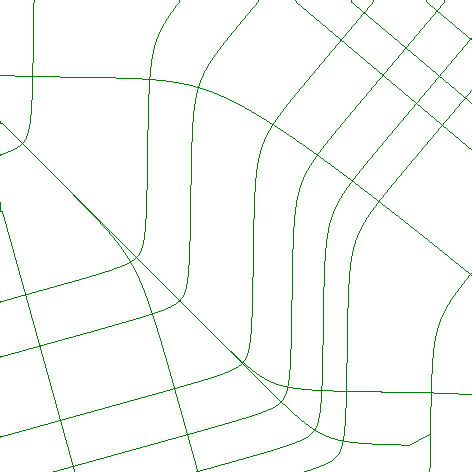
\includegraphics[width=4in]{images/linear.pdf}}
    \caption{Streamline tracing near road merging}
\end{figure*}

\begin{figure*}[t!]
    \centering
    \begin{subfigure}[b]{2.4in}
        \fbox{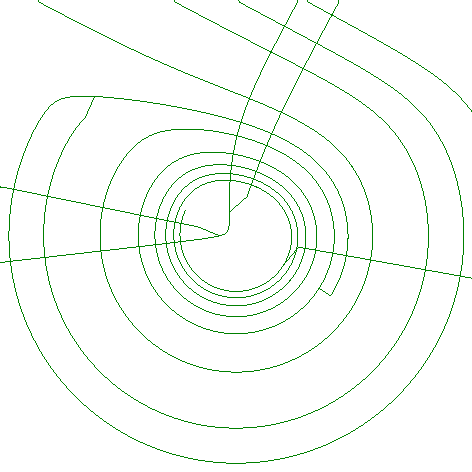
\includegraphics[width=\textwidth]{images/cycle_nodetection.pdf}}
        \caption{without cycle detection}
    \end{subfigure}
    \hspace{20pt}
    \begin{subfigure}[b]{2.4in}
        \fbox{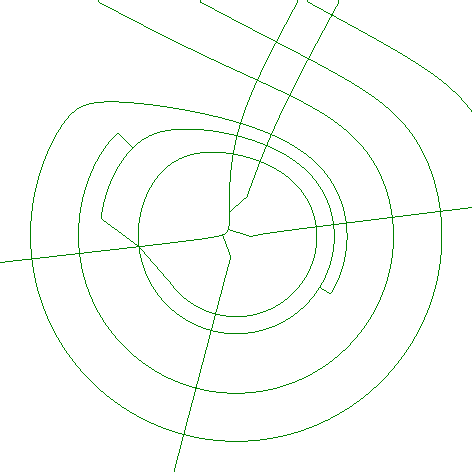
\includegraphics[width=\textwidth]{images/cycle_detection.pdf}}
        \caption{with cycle detection}
    \end{subfigure}
\caption{Streamline tracing cycle detection}
\label{fig:cycles}
\end{figure*}

\subsection{Seed Placement}\label{sec:seedpoints}
To begin constructing a streamline, one must choose a seed point—--an initial
coordinate in 2D space from which the streamline is traced. In practice, the
matter of carefully choosing seed points is very important in generating an
evenly spaced configuration of roads. We investigated three methods of placing
seed points.

\paragraph{Random}
Purely random placement of seed points generally results in both clusters of
roads which are too close together and large gaps between roads.

\paragraph{Furthest-Point}
In the furthest-point placement, we place each new seed point within the bounds
of the space such that the distance to all existing streamlines is maximized.
As a simplifying heuristic for this method, we generate a number of random
candidate seed points which is small compared to the infinite number of
possible seed points and choose the one furthest from all existing streamlines.
In practice, this offers a significant improvement over the random seed
placement, and results in a more even distribution of streamlines.

\paragraph{$\chi^2$ Streamline Spacing}
However, even choosing well-spaced seed points will not necessarily result in
an even distribution of streamlines, since two well-spaced seed points can
result in two streamlines which quickly converge. Therefore, we introduce a
third method. To assess how evenly spaced a set of streamlines is, we will
generate a set of discrete points evenly spaced along each streamline, place
these points into $n\times n$ equal-sized buckets covering the bounds of the
space, and perform a chi-squared goodness of fit test on distribution of points
across buckets:
\[
    \chi^2 = \sum_{i=1}^{n}\sum_{j=1}^n \frac{(O_{ij}-E_{ij})^2}{E_{ij}}
\]
where $n$ is the number of buckets along each axis, $O_i$ is the observed
number of points in the bucket at position $(i,j)$, and $E_i=\frac{m}{n^2}$ is
the expected number of points in each bucket, assuming a uniform distribution
and $m$ is the total number of points in the space.

We will choose the seed point whose corresponding streamline, when added to the
existing set of streamlines, optimizes the evenness of streamline placement,
according to the above metric. As with the previous method, we employ a
simplifying heuristic, generating a relatively small set of candidate seed
points, tracing a streamline from each, determining which streamline results in
a more even field of streamlines, and adding it to the existing set of
streamlines.

\section{Assessment}
We set out to achieve two goals: modularity and expressiveness. In this section
we will examine the extent to which these goals were achieved.

\subsection{Modularity and Extensibility}
In Section \ref{sec:seedpoints}, we outlined three methods of seedpoint
placement: random, furthest-point, and $\chi^2$ even spacing. All three are
implemented by functions in the \texttt{Streamline} module, and follow a
similar template. Extending this module with other methods is as simple as
implementing a new function with the same type signature as one of the existing
seed-placement functions, adding a new value constructor to the datatype
\texttt{PlacementMethod}, and adding a new case to the function
\texttt{placeStreamlines} to match the new value constructor. The purity of
functions in a language such as Haskell makes it simple to drop in replacements
for existing functions because one does not have to consider possible side
effects, but only the types of the inputs and output.

In order to detect intersections between streamlines as they are traced, we
defined the \texttt{NearestNeighbor} module to implement a data structure which
stored a set of 2D points and could be queried to determine which of the stored
points was closest to the query point. This is implemented using a type family,
with an instance utilizing a blocked 2D array implementation. This instance was
sufficient for testing purposes, but is currently the performance bottleneck in
streamline tracing. A new instance of the \texttt{Storage} type family could
easily be defined in accordance with the type signature to provide a more
efficient representation. For example, an instance of the type family
implementing a k-d tree could offer improved performance. This well-defined
abstraction boundary makes this aspect of our pipeline very easily extensible.

\subsection{Expressiveness}
As our work was not a complete reimplementation of the system described in
\cite{chen}, it is difficult to compare the relative expressiveness of our
Haskell code with the \cpp code of the original implementation. However, we
will present one comparison of functions from our respective implementations
with significantly overlapping functionality. Our Haskell code for calculating
the eigenvectors for a tensor can be found in Figure \ref{fig:evecs}. The
reader may note the close correspondence between the body of these functions
and the mathematical formulas used for calculating eigenvectors in Section
\ref{sec:eigenvectors}.  While the 75-line function
\texttt{cal\_eigenvecs\_onevert\_quad} in Chen's implementation is documented,
we found it difficult to determine its side effects. We found that a functional
language without mutable state or side effect made it significantly easier to
fully understand the behavior of functions.  In contrast, even well-written
code in \cpp or another language in the imperative paradigm can be difficult to
understand, because the possibility for side effect requires the reader to have
an understanding of any part of the system that the function can affect. In
practice can make the effort to understand any small part of a large codebase
much greater.

\begin{figure*}[t!]
\begin{Verbatim}[frame=single]
-- returns a tuple of the (larger, smaller) eigenvectors of a tensor
eigenvalues :: Tensor -> (Float, Float)
eigenvalues (Tensor a b d) =
let eval = sqrt (a*a + b*b)
in  (eval, (-1)*eval)

-- returns a tuple of the (major, minor) eigenvectors for a tensor
eigenvectors :: Tensor -> (V2.Vector2, V2.Vector2)
eigenvectors (Tensor a 0.0 d) =
if a > d then (V2.Vector2 1 0, V2.Vector2 0 1)
   else (V2.Vector2 0 1, V2.Vector2 1 0)
   eigenvectors (Tensor a b d) =
     let (eval1, eval2) = eigenvalues (Tensor a b d)
         mkEvec eval    = V2.Vector2 1 ((eval - a) / b)
     in (mkEvec eval1, mkEvec eval2)
\end{Verbatim}

\caption{Haskell implementation of eigenvector calculation (from
            \texttt{Tensor.hs})}
\label{fig:evecs}
\end{figure*}

\section{Conclusion}
In this paper we have presented the underlying mathematics and functional
implementation of the work described in \cite{chen}, with the goals being that
a functional implementation would readily express the mathematics, and provide
modularity that the imperative implementation provide in \cite{chen} could not.
We believe that, due to the focus on expressibility and modularity that an
individual looking to understand the pipeline will find our code undestandable
and approachable, and lend itself to be easily extended. We hope that our work
will motivate a greater use of functional languages in future efforts in the
research of new procedural algorithms.

\bibliographystyle{alpha}
\bibliography{references}

\end{document}
